\chapter{Model Construction}
\label{chap:ModelConstruction}

\section{Preliminaries}
\subsection{High-level Approach}
The purpose of WoB is to calculate granular service demand for a particular timetable based on supplied origin-destination (O-D) trip data. The high-level algorithm of the WoB simulation consists of the following loop:

\begin{SingleSpacing}
    \begin{enumerate}
        \item Initialise the "crowding cost" of each transit service in the network to 0.
        \item For each set of agent journeys in the input data, determine the transit services used, taking the crowding of services into account, and record the agents as populating the proportion of any trips they use.
        \item Based on the calculated utilisation, determine a "crowding cost" to associate with each transit service.
        \item Go to step 2, or output results and halt.
    \end{enumerate}
\end{SingleSpacing}

This chapter describes how these high-level steps are implemented in WoB, with the required practical considerations. Step 2 of the above loop is a pathfinding problem, which requires the ability to represent a timetabled transit network in computer memory and efficiently traverse it, while maintaining a record of agent populations on services. Step 3 is based on the idea of a crowding model and cost function, which is briefly described here but explored in more detail in \refandname{chap:ModelSpec}. Step 4 requires iterative replanning logic and a halting condition, which is also described in this chapter.

Besides this high-level loop, there is additional auxiliary functionality that is required to support the core algorithm. The input and output data to the algorithm must have a specification and import and export processes. A graphical user interface (GUI) was also created to support the accessibility objective of the project.

\subsection{Existing Work}
The following is a brief overview of the work WoB is built upon. WoB is a comprehensive extension of the simulation framework completed in the semester one research report ``Simulating Melbourne's Metropolitan Train Network using Agent-Based Modelling Techniques'', which should be referred to for the full implementation details \cite{benjaminsutherlandSimulatingMelbournesMetropolitan2024}.

\subsubsection{Network Layout}
Public transport timetables are represented in computer memory by a series of stops, routes, trips and stop times by importing and processing a GTFS dataset, which is generally officially provided but can also be converted from other formats. The trips in the GTFS dataset are filtered to only select those running on a given day, then the stop times for each trip are serialised into a linear array, grouped by route for fast lookup.

The network layout allows fast traversal of trips by grouping subsequent stop times together in memory, and fast lookup of stops, routes and trips using integer indices. Connections, or the consecutive pairs of departure-arrival stop times are also generated despite technically being redundant information, because they can be used by alternate pathfinding algorithms.

\subsubsection{Pathfinding Algorithms}
The simulation framework implemented the RAPTOR pathfinding algorithm with single-criterion support. In this research RAPTOR was extended to the multi-criteria problem to support agent replanning. 

\subsubsection{Assigning Passenger Counts}
Once the journeys for a group of agents has been generated, the service demand can be calculated. To record passenger counts, the same lookup logic used for stop times is repurposed. A buffer with the same length as the stop times array is initialised to zero, then the number of passengers on the train between stop time $i$ and stop time $i+1$ is recorded in the passenger count buffer at the index of stop time $i$. Thus the passenger count is calculated at the granularity of the connection. Also note that this algorithm results in each trip record being terminated by a count of 0. To allow for optimisations based on parallelisation, passenger counts use atomic integer types. 

During this stage, the passenger count (an absolute, linear record) can be converted into a crowding cost (a subjective, non-linear value) using a crowding cost function. The existing work used a simple exponential crowding model, as more advanced models were beyond the scope of the project. In this project we take a much deeper look at different crowding functions in \refandname{chap:ModelSpec}.

\subsubsection{Visualisation}
To display agent movements through the network, the output of the simulation is exported in a format that can be consumed by a visualisation library. The Deck.gl JavaScript web framework \cite{VisglDeckGl2024} was chosen for its simple programming interface and interactivity. Each connection in the network was exported with its temporal and geographical information, and associated crowding cost. The Deck.gl library then rendered and animated each trip in the network on an interactive map interface.

\subsection{Extension to Full Model}
To extend the framework to the full model, the following features were added.
\begin{SingleSpacing}
    \begin{enumerate}
        \item Data import
        \item Multi-criteria pathfinding 
        \item Crowding cost functions 
        \item Iterative replanning
        \item User interface
    \end{enumerate}
\end{SingleSpacing}

The various crowding cost functions used by the model are discussed in \Cref{chap:ModelSpec}.
Additionally, the performance of the model is investigated in \Cref{sec:Performance}.

\section{Data Import}
\label{sec:DataImport}
The patronage data that drives the simulation is a set of journeys taken across the network over a day. A sample is shown in \autoref{tab:SimInput}. Due to the large size, this is stored and imported as a parquet file \cite{apachesoftwarefoundationParquet2024}. The method of processing the input data used in the case study portion of this paper is discussed in \Cref{chap:CaseStudy}.

\begin{table}[ht]
    \centering
    \caption[Sample input to simulation framework]{Sample input to simulation framework, based on the case study data for Melbourne. This table displays the specific format the WoB model application consumes.}
    \begin{tabular}{cllc}
        Origin         & Destination       & Departure Time  & Count \\ \hline
        Flinders Street & Williams Landing    & 00:00:00       &           4 \\
        Flinders Street & Mordialloc          & 00:00:00       &           1 \\
        Glenferrie      & Flinders Street     & 00:00:00       &           1 \\
        Flinders Street & Ginifer             & 00:00:00       &           2 \\
        Flinders Street & Lilydale            & 00:00:00       &           1 \\
        \multicolumn{4}{c}{\vdots}\\
        Footscray       & Parliament              & 08:30:00       &           1 \\
        Glen Iris       & Parliament            & 08:30:00       &           1 \\
        Essendon        & Parliament             & 08:30:00       &           1 \\
        Ferntree Gully  & Southern Cross       & 08:30:00       &           4 \\
        Box Hill        & Southern Cross       & 08:30:00       &           7 \\
        \multicolumn{4}{c}{\vdots}\\
        Parliament          & Hoppers Crossing &  17:15:00       &           2 \\
        Flinders Street     & Glenroy          &  17:15:00       &           3 \\
        Flinders Street     & Hoppers Crossing &  17:15:00       &           5 \\
        Southern Cross      & Hoppers Crossing &  17:15:00       &           5 \\
        Melbourne Central   & Keilor Plains    &  17:15:00       &           2 \\
        Parliament          & Keilor Plains    &  17:15:00       &           3 \\
        \multicolumn{4}{c}{\vdots}\\
    \end{tabular}
    \label{tab:SimInput}
\end{table}

An important property of this data is that the entries can be grouped by origin and departure time (\autoref{tab:GroupedSimInput}). For example, Melbourne's City Loop stations can group together many trips (the whole dataset going from over 300,000 entries to just under 14,000 groups), but this property applies to any network with central hub stations. A significant optimisation can be implemented by only running a single multi-destination query per group, rather than per entry. 

\begin{table}[ht]
    \centering
    \caption[Sample grouped input to simulation framework]{Sample grouped input to simulation framework.}
    \begin{tabular}{cll}
        Origin         & Departure Time  &  [Destination Count, ...] \\\hline
        Flinders Street & 00:00:00       &  [Williams Landing 4, Mordialloc 1, ..]\\
        Glenferrie      & 00:00:00       &  [Flinders Street 1]\\ 
        \multicolumn{3}{c}{\vdots}\\
        Footscray       &  08:30:00       &           [Parliament 1] \\
        Glen Iris       & 08:30:00    & [Parliament 1]      \\
        Essendon         & 08:30:00   & [Parliament 1]      \\
        Ferntree Gully & 08:30:00     & [Southern Cross 4]    \\
        Box Hill      & 08:30:00  & [Southern Cross 7]         \\
        \multicolumn{3}{c}{\vdots}\\
        Parliament           &  17:15:00  & [Hoppers Crossing 2, Keilor Plains 3] \\
        Flinders Street      &  17:15:00  & [Glenroy 3, Hoppers Crossing 5] \\
        Southern Cross       &  17:15:00  & [Hoppers Crossing 5] \\
        Melbourne Central    &  17:15:00  & [Keilor Plains 2] \\
        \multicolumn{3}{c}{\vdots}\\
    \end{tabular}
    \label{tab:GroupedSimInput}
\end{table}

\section{Multi-Criteria Pathfinding}
A core component of the replanning algorithm is determining routes for agents based on more than just earliest arrival time. For our model to take crowding into account, agents must be able to change their routes based on the crowding of services. 

This technique is called "multi-criteria pathfinding", where an additional cost is taken into account when determining routes. More precisely, the multi-criteria problem asks for a full Pareto-set of journeys leaving a given origin stop no earlier than a given departure time \cite{dellingRoundBasedPublicTransit2012}. 

A Pareto-set is a set in which each element does not dominate any other - i.e., a trade-off must be made to choose any option over any other. A solution dominates another solution if it is better in all criteria, and strictly better in at least one \cite{bergerAcceleratingTimeDependentMultiCriteria2009}.

As such, the multi-criteria version of the pathfinding algorithm returns a set of different journeys, each with a different associated arrival time and crowding cost. A cost function is applied to each journey to determine which journey a particular agent will take (this process is elaborated upon in \Cref{sec:FinalJourneyCostFunction}).

The fundamental difference between single-criterion and multi-criteria algorithm designs is the bookkeeping method. During a single-criterion run, only the earliest arrival at a given stop need be recorded, corresponding to a single journey. However, during a multi-criteria run, at each stop, a set of earliest arrival time and crowding cost pairs (called "labels") must be stored, which is considerably more complicated. In single-criterion pathfinding, a simple assignment operation is used to update the earliest arrival time at a stop based on a newly found trip. For multi-criteria, a new label must only be added to the list if it is non-dominated in the set, and then any newly dominated labels in the set must be subsequently removed.

This model technically implements a sub-problem of multi-criteria pathfinding by only considering two criteria, arrival time and crowding cost. In general, multi-criteria pathfinding can find Pareto-optimal journeys from any number of criteria, but our implementation makes use of some optimisations that can only be made for the dual-criteria case.

\subsection{Using Bags to Store Labels}
The data structure that is generally used for recording these Pareto-optimal sets is a "bag", which is a generic term for a set with specific allowed operations. Most general solutions involve dynamically allocating memory in a resizable array, but because these bag operations are extremely frequent during pathfinding they must be as efficient as possible \cite{dellingRoundBasedPublicTransit2012}. We can set an upper bound on the number of stored journeys, which discards labels based on some criteria and allows us to statically inline the array. The label with the latest arrival time is discarded as these are generally the least realistic (going to extreme lengths to avoid crowded services) but this could be replaced with a specific utility calculation.

% The literature talks about a special case that can be optimised - when the other criteria is a discrete set like fare zones. These can be represented by a bit-set, and checking for domination is merely a bitwise AND operation and set-union a bitwise OR.

The implementation of our bag data structure is designed to take advantage of the ordered nature of dual-criteria labels. Each label has an associated arrival time and crowding cost property. Labels in a bag cannot have the same value for either property, because that would imply domination (if they had the same arrival time, only the label with the lower crowding cost should be kept and vice versa). Additionally, if the labels are sorted in ascending order by arrival time, then they are also sorted in descending order by crowding cost (if the arrival time increases, the crowding cost must decrease). 

The set insertion operation works as follows. First, the array is partitioned based on whether the arrival time is earlier or later than the new label (more precisely, the first partition contains all labels with earlier or equal arrival time, and the second contains all labels with later arrival times). This step is achieved with a simple linear search, but a binary search could be used for larger bag sizes. Then, all labels in the first partition are checked to see if they dominate the new label, in which case the new label is discarded. All labels in the second partition are checked to see if they are dominated by the new label, in which case they are discarded. If the bag is full, the last label (latest arrival time) is removed. The new label is then inserted at the partition point. Bags often need to be merged, which amounts to the repeated insertion of labels from one bag into another.

\subsection{Extending from Single-Criterion}
While the bag data structure is a novel implementation, the single-criterion version of RAPTOR was extended to handle multi-criteria queries based on the description in the original paper by Delling et al. \cite{dellingRoundBasedPublicTransit2012}. Much of the route iteration logic is the same, so it was refactored out into a common function to be used for both single- and multi-criteria queries. The multi-criteria algorithm adds labels to each stop's bag by iterating along each route and keeping a record of the labels of the previous stop. These labels are updated by applying a train connection to them, i.e. setting the arrival time to the next stop and adding the associated crowding cost. They are then merged into the current stop's bag, and the previous round's labels are merged into the route bag.

\subsection{Determining the Preferred Journey}
\label{sec:FinalJourneyCostFunction}
Once the bags of labels corresponding to each stop have been filled, one of the many Pareto-optimal journeys must be chosen for the agent to follow. A general cost function (as opposed to a crowding cost function) is supplied as part of the query which can assign a single cost value to any given multi-criteria label. This means that a single label can be chosen from a bag by choosing the label with the minimum cost, as ascribed by the cost function. This function has the form 
\begin{equation}
    f(t_a, c) = (t_a - t_d) + c_u \times c 
    \label{eqn:cost_utility}
\end{equation}
where $t_a$ and $c$ are the label's arrival time (in seconds) and crowding cost respectively, $t_d$ is the journey query departure time and $c_u$ is the relative crowding cost utility. Each pathfinding query defines $t_d$ and $c_u$ as constants. The $c_u$ constant determines how a given crowding cost value is compared to a given time value. For example, if $c_u = 1$ then every unit of crowding cost equates to one second of travel time utility, and an agent might choose to take a one second slower journey per unit of crowding cost incurred in a faster journey. Taken together, minimising this function equates to minimising the travel time and the crowding cost.

A "leg" is a contiguous set of connections on the one trip, so a journey may contain multiple legs with transfers at stations in between. To reconstruct each leg of the journey, each label in each stop's bag also has a field that records the boarding data for that journey, i.e. which trip departing at what stop would need to taken to arrive at the label's arrival time, incurring the label's crowding cost. Once this leg has been recorded, the bag of the boarded stop is inspected similarly to determine the best label. Every subsequent bag inspection also filters labels to ensure their arrival time is before the departure time of the previous leg (previous in terms of processing order, but next in terms of journey order). This process appends the legs in reverse order, so the final step is to reverse the list of legs before returning them.

\subsection{Multi-destination Extension}
As described in \Cref{sec:DataImport}, the journeys are grouped by origin and departure time. A multi-destination query can be run that finds the corresponding set of journeys to a set of destinations from a given origin and departure time. Because there is a significant amount of overlapping work between queries with the same origin and departure time, using multi-destination queries is an important optimisation. However, to run a multi-destination query the "target pruning" optimisation from standard RAPTOR needs to be removed. This optimisation prevents any stops from being updated to arrival times later than the arrival time at the target stop, which allows the algorithm to exit earlier. However, in our case, we can conditionally enable this optimisation in the case of a single destination, and otherwise explore the entire network. A journey path can then be calculated for each destination.

\section{Iterative Replanning}
To ensure agents take their own crowding preferences into account, the simulation is split into rounds, with each round using the results of the previous round to calculate specific demand for services. This approach has the significant advantage that \emph{during} each round each agent is completely independent. During each round, the order in which the agents are processed is irrelevant, which allows the agent processing to be trivially parallelisable. As such, this the model can make good use of modern multi-core processors which can be used to speed up simulation time.

The first round calculates the routes agents would take if the network was completely empty. This can be done with the single-criteria RAPTOR algorithm, so this round is very fast. Subsequent rounds use multi-criteria RAPTOR to recalculate the agent journeys based on the previously calculated crowding cost. 

\subsection{Trip Capacities}
To account for variations in train capacity across the network, WoB has an optional CSV file input for trip capacities, which specifies seated and standing capacities for each trip defined in the GTFS. These capacity values are passed as parameters to the crowding cost function. If this file is not specified, then default capacities can be selected in the user interface.

\subsection{Halting and Convergence}
\label{subsec:convergence}
Each round uses the previous round to inform the journeys agents take, but the halting condition remains undefined. In general, the difference from the previous round can be used to determine if more rounds are required. Some similar types of iterative problems perform this automatically and will halt when the round result difference falls below a set threshold. However, as shown in \Cref{fig:simulation_convergence}, we found in the case of our model that with calibrated crowding settings the round converged within 3 rounds. Therefore, WoB provides the number of rounds as a configurable parameter that can be tweaked as desired. 

\begin{figure}[ht]
    \centering
    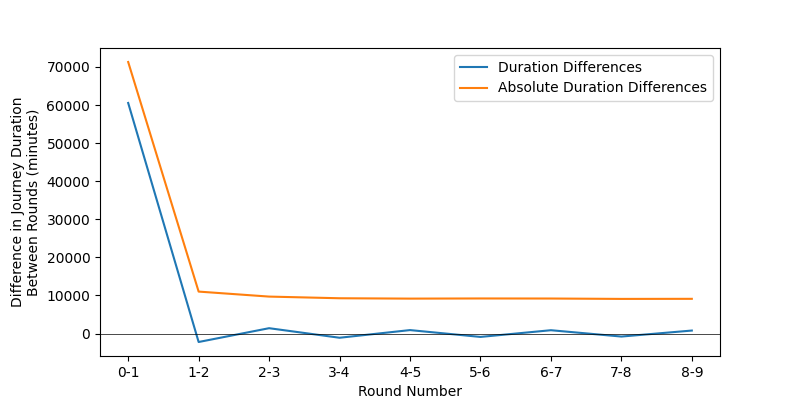
\includegraphics[width=\linewidth]{images/Construction/convergence.png}
    \caption[Simulation convergence]{Graph of the differences in the total simulated journey time between simulation rounds. The duration difference is calculated by summing the difference in the journey duration between rounds over every agent. The absolute duration difference is the same process, but sums the \emph{absolute value} of the difference.}
    \label{fig:simulation_convergence}
\end{figure}

\section{Graphical User Interface}
A key aim of the model is to be as accessible as possible. The existing simulation framework only had a command-line interface, which was difficult to use without training. A Graphical User Interface (GUI) for the model was created to facilitate creating a transport network layout from a GTFS dataset, importing patronage data and configuring simulation parameters \cite{mobilitydataReferenceGeneralTransit2024}.

Our user interface implementation uses Tauri, a library for embedding web-based user interface technologies in a desktop application with interoperability with code compiled natively \cite{TauriappsTauri2024}. To simplify the web design component, we opted to use the Svelte \cite{SveltejsSvelte2024} framework as the front-end, which provides a modular way to design reactive interfaces.

A crucial element of the GUI implementation is allowing the web-based front-end to communicate with the native back-end. This communication is required for tasks such as beginning the simulation process and receiving the results so they can be visualised. The Tauri inter-process communication (IPC) component provides this functionality.

\subsection{Inter-process Communication}
The Tauri framework allows code written in the programming language Rust (such as the simulation logic) to be invoked by JavaScript running in the GUI. Generally, this is linked to a button press e.g. the "Run Simulation" button gathers the selected parameters and passes them to a Rust function to begin the simulation.

Usually, the parameters are serialised into a JSON string (as is standard with JavaScript interoperability), which are then deserialised by the Tauri IPC and passed to the Rust function. Returning values to JavaScript works similarly. For parameters such as crowding function coefficients, this works perfectly, but for passing a large amount of binary data (such as input data files and the simulation results) the round-trip JSON serialisation adds significant overhead. While there is no alternative in version 1.0, Tauri 2.0 was released as stable on October 2nd 2024 with raw binary request/response functionality (this project was largely developed using the release candidate version of Tauri 2). This allows an array of bytes to be transferred directly, skipping the JSON serialisation and deserialisation step, and leads to a significant speedup.

\subsection{Visualisation}
The Deck.gl-based visualisation of train movements colourised by each services' crowding from semester one was embedded in the GUI \cite{benjaminsutherlandSimulatingMelbournesMetropolitan2024}. 

\section{Data Export}
There are four types of data export schema that encapsulate the simulation results in different ways; agent counts, journeys, legs and transfers. 

\subsubsection{Agent Counts}
The agent count file is a record of the number of agents between each pair of adjacent stations for every train service running that day. This is the primary output that allows general network crowding to be analysed. 

\begin{table}[ht]
    \centering
    \caption[Sample simulation agent counts]{Sample simulation agent count output from the Melbourne case study dataset.}
    \begin{tabular}{lcllc}
         Trip ID & Time & Departure & Arrival & Count\\\hline
         82.T0.2-GLW-mjp-6.9.H & 07:38:00 & Jordanville & Mount Waverley& 36\\
         82.T0.2-GLW-mjp-6.9.H & 07:40:00 & Mount Waverley & Syndal& 24\\
         82.T0.2-GLW-mjp-6.9.H & 07:43:00 & Syndal & Glen Waverley & 9\\
        \multicolumn{4}{c}{\vdots}\\
    \end{tabular}
    \label{tab:AgentCountsFileStructure}
\end{table}
\subsubsection{Agent Journeys}  
The agent journeys file is a record of each simulated journey with the number of agents undertaking it, the origin and destination station, the departure and arrival time, as well as the specific departure and arrival trip, the number of transfers made during the journey and the total cost due to crowding for the journey. This output enabled agent traversal behaviours to be analysed, as demonstrated in \Cref{chap:CaseStudy}. 

\subsubsection{Agent Legs}
The agent legs file is similarly formatted, but contains a record for every "leg" of every simulated journey (i.e. each contiguous trip between transfers) an agent group makes. This output type gives the most comprehensive picture of the network service demand, and was used to validate the model against the input data in \Cref{chap:CaseStudy}, \Cref{sec:validation}.

\subsubsection{Agent Transfers} 
The agent transfers file only keeps a record of agents that make a transfer on the network. Each entry lists an incoming trip, an arrival time, a transfer station, a departure time and an outgoing trip, along with the number of agents that made the transfer. These outputs enabled transfer behaviours to be analysed, as demonstrated in \Cref{chap:CaseStudy}. 

\section{Performance}
\label{sec:Performance}

\begin{figure}[ht]
    \centering
    \begin{tikzpicture}
        \begin{axis}[
                axis lines = left,
                xlabel = Round \#,
                xmin=0,
                ylabel = Processing Time (s),
                ymin=0,
                legend pos=south east,
            ]
            \addlegendimage{empty legend}
            \addlegendentry{\hspace{-.6cm}\textbf{Bag size}}
            \addplot[smooth,mark=*,red] table [x=round_number, y=t_2, col sep=comma] {data/performance5.csv};
            \addlegendentry{2 }
            \addplot[smooth,mark=*,blue] table [x=round_number, y=t_3, col sep=comma] {data/performance5.csv};
            \addlegendentry{3 }
            \addplot[smooth,mark=*,green] table [x=round_number, y=t_4, col sep=comma] {data/performance5.csv};
            \addlegendentry{4 }
            \addplot[smooth,mark=*,orange] table [x=round_number, y=t_5, col sep=comma] {data/performance5.csv};
            \addlegendentry{5 }
        \end{axis}
    \end{tikzpicture}
    \caption[Graph of model performance]{Model performance for each round with different multi-criteria bag sizes (i.e. the maximum number of journey options considered at once). These numbers were produced on the Melbourne instance (\Cref{chap:CaseStudy}) on a quad-core laptop computer at 3.7GHz, with a peak memory usage of 2.5GB.}
    \label{fig:ModelPerformance}
\end{figure}

The WoB model is designed with performance in mind. This means that at each stage of the implementation process, the data structures and algorithms were optimised as much as reasonably possible. As shown in \Cref{fig:ModelPerformance}, which is generated based on the Melbourne case study data of almost 500,000 agents (\Cref{chap:CaseStudy}), the time to perform a single round was always less than or equal to 4 seconds, and the time to perform all 8 rounds considering 5 journey options at a time was 27.6 seconds. Round 0 is consistently the fastest because it does not optimise for crowding, instead generating the baseline crowding values for subsequent rounds. The performance converges to a stable value after round 2 for all bag sizes, with there being a slight performance penalty for larger bag sizes. The peak memory usage for running 8 simulation rounds was 2.5GB, which is a reasonable memory budget for modern consumer laptops \cite{SpecificationsPersonalComputers}.

